%\renewcommand{\lastmod}{April 29, 2020}

\chapter{Absorption}




\section{Tasks}

\begin{itemize}
\item Get acquainted with the different measures for absorption and how they relate. Starting from the experimental values in the following papers, calculate all other measures.

\begin{tabular}{ll}
InGaAs quantum dots & \cite{Borri:2002p139}, last page  \\
CdSe nanocrystals & \cite{Jasieniak:2009er}, Fig. 2 and 3 \\
xanthene dye & \cite{Kastrup:2004p1737}, Fig. 4d   \\
MEH-PPV conjugated polymer  & \cite{Hou:2017jm}, Fig. 3 \\
\end{tabular}


\item Get a feeling for typical absolute values and compare them to relevant  other quantities, such as geometrical size, bond lengths, transition rates etc. Sometimes it makes sense to factor out some constants and compare only then.
\item Why are there so many different measures for absorption? Find use cases where it makes especially sense to use one measure and not the others.

\end{itemize}







%\section{Experiment}
\section{Experimental technique}

An UV/VIS spectrometer measures the  power $P$ transmitted through a cuvette of optical path length $L$ and compares it to the power $P_0$ in a reference path. In most cases, also here, the reference path holds a cuvette containing  the plain solvent. The transmission $T = P / P_0$ is converted into the absorbance $A = - \log_{10} T = - \log_{10} ( P / P_0)$. The data set gives absorbance as function of wavelength.

\begin{marginfigure}
\inputtikz{\currfiledir/uvvis}
%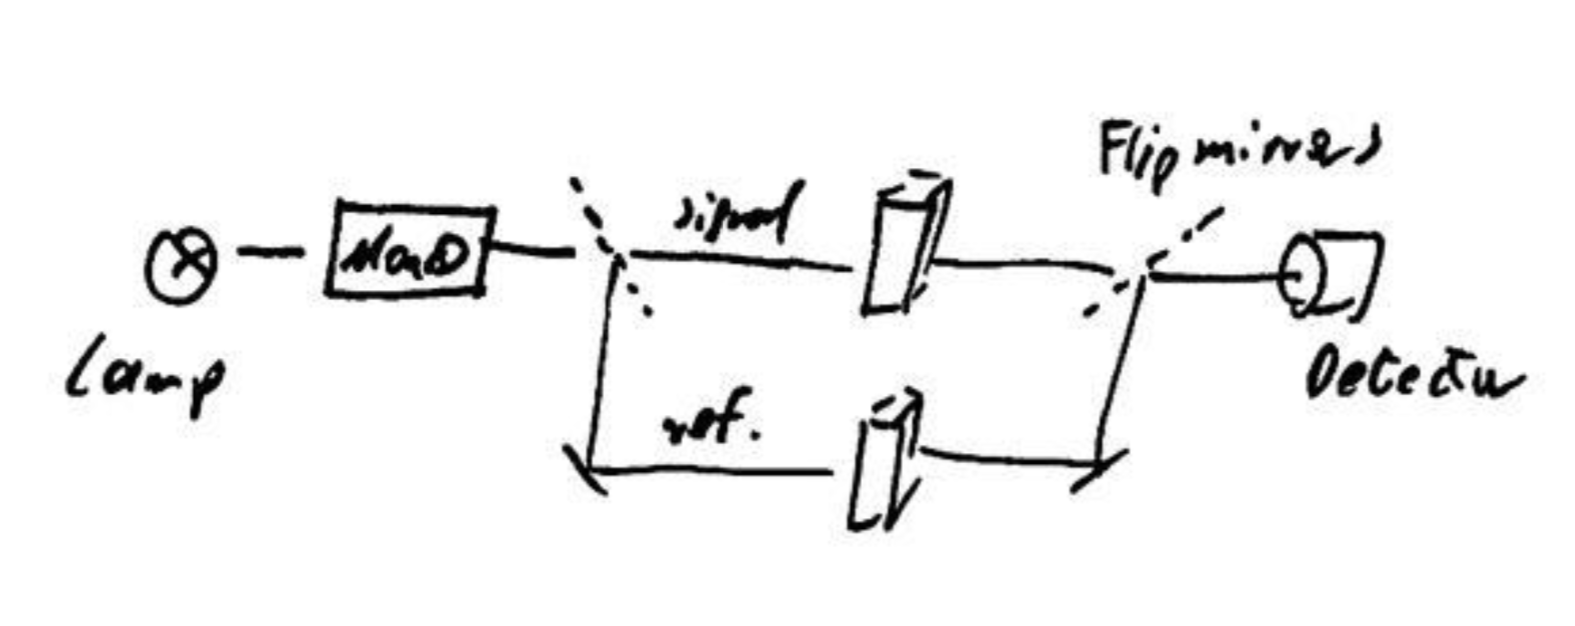
\includegraphics[width=\textwidth]{\currfiledir/uvvis.png}
\caption{Sketch of a UV/VIS spectrometer}
\end{marginfigure}



Grating spectrometers use an entrance slit to define the spectral resolution $d \lambda$, which is independent of the actual wavelength $\lambda$, as can be seen when inspecting the   angular dispersion relation of a grating. Due to the reciprocal relation between wavelength and frequency or energy, the spectral resolution in units of energy $d \nu$ is not constant anymore.




\section{Lambert-Beer law and the absorption coefficient}

The transmitted power drops exponentially with  concentration $C$ and  path length $L$
\begin{equation}
 P = P_0 \, 10^{- \epsilon\, C \, L}
\end{equation}
where $\epsilon$ is the (decadic) molar absorption\sidenote{The difference between abortion and extinction will be discussed elsewhere.} coefficient. We stick here to a base of $10$, 
so that the absorbance or optical density equals 
\begin{equation}
 A = \epsilon\, C \, L \quad.
\end{equation}
However, similar definitions with a base of $e$ are used sometimes. Our choice leads to the appearance of factors of $\ln(10)$ every now and then. The concentration is typically given as molarity (1 M = 1 mol/l), and lengths for practical reasons in centimeter
so that the molar absorption coefficient has the unit 1/(M  cm). As we are concerned with spectroscopy the molar absorption coefficient $\epsilon$ depends of course on the wavelength or frequency of light.

\section{Absorption cross section}


The interaction cross section $\sigma$ of a process is an imagined area around the particle, which, when hit by a photon, triggers the considered process. When a photon hits on the absorption cross section $\sigma_{\text{abs}}$ of a molecule it will be absorbed. If it does not hit it will pass unperturbed. All details of the physics are summarized in the area, which makes it easy to relate the absorption cross section with the absorbance. 
\begin{marginfigure}
\inputtikz{\currfiledir/crosssection}

%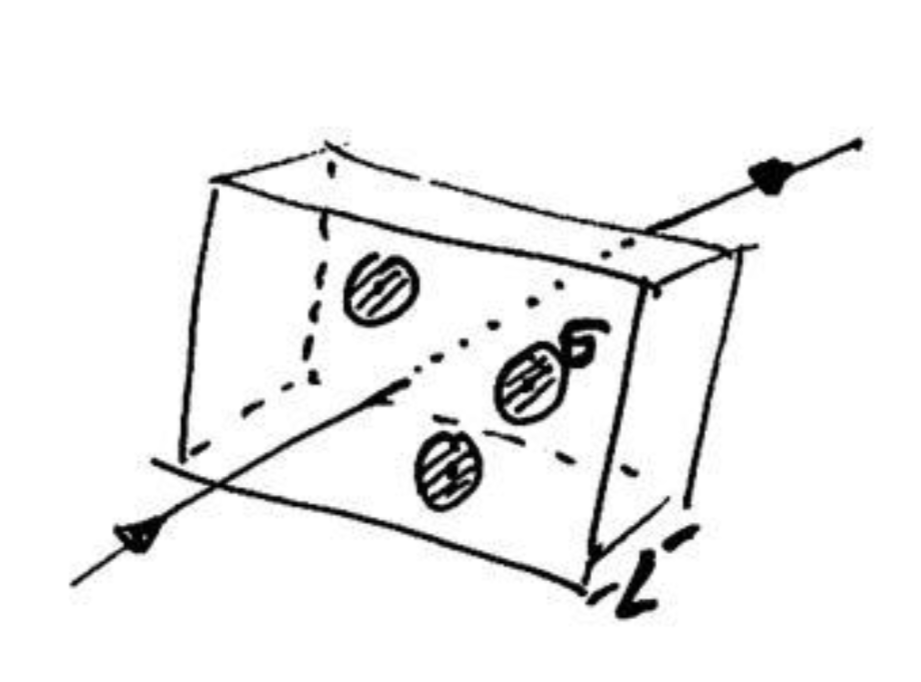
\includegraphics[width=\textwidth]{\currfiledir/crosssections.png}
\caption{Sketch  disks hit by rays}
\end{marginfigure}


We consider randomly arranged molecules of molar concentration $C$ in a thin slab of thickness $dx$. The probability that a photon is absorbed in this slab is
\begin{equation}
 1 - T =1 -  10^{- \epsilon\, C \, dx} \approx \ln (10) \; \epsilon\, C \, dx \quad .
\end{equation}
In comparison, when each molecule has an absorption cross section $\sigma_{\text{abs}}$, we get an absorption probability 
\begin{equation}
 1 - T = \sigma_{\text{abs}} \, C \, N_A \, dx
\end{equation}
where $N_A = 6.022 \cdot 10^{23}$~{1/mol} is the Avogadro number.  We also made the Born approximation, i.e., that multiple interactions can be neglected, or the absorption cross sections do not overlap, which is equivalent to the approximation made above to remove the exponential function.  We thus find
\begin{equation}
 \sigma_{\text{abs}}(\omega) =  \frac{\ln(10)}{ N_A } \, \epsilon(\omega)
\end{equation}
which has the unit of an area. As the  molar absorption coefficient $\epsilon$  also the absorption cross section $\sigma_{\text{abs}}$ depends on the wavelength of light. If no wavelength is given, the value at the peak of the spectrum is meant.


\section{Lorentz oscillator and oscillator strength}


\begin{marginfigure}
%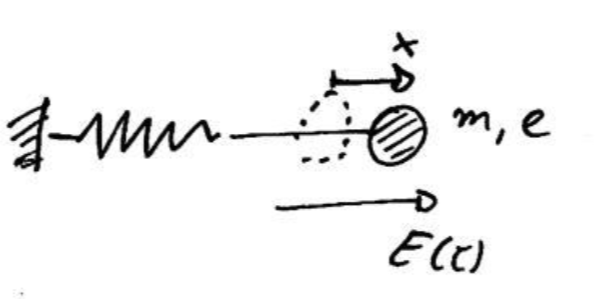
\includegraphics[width=\textwidth]{\currfiledir/lorentz.png}
\inputtikz{\currfiledir/mass_spring}

\caption{A Lorentz oscillator}
\end{marginfigure}


The Lorentz oscillator is a simple classical model to describe the interaction of light and matter. A mass $m$ of charge $+e$ is connected to a spring. The oscillator has an angular eigen-frequency $\omega_0$ and a damping $\gamma$. It is driven by an external electrical field $E(t) = E_0 \exp(i \omega t)$. The differential equation for the position $x$ reads
\begin{equation}
  \ddot{x} + 2  \gamma  \dot{x} + \omega_0^2 x =  \frac{e}{m} E_0 e^{i \omega t}
\end{equation}
This results in a steady-state solution of \sidenote{check: should be $-i\gamma$ for Lorentz osci}
\begin{equation}
  x(t) = \frac{e}{m}  \frac{1}{\omega_0^2 - \omega^2 + 2  i \gamma \omega } \, E_0 e^{i \omega t} 
\end{equation}
In the case of small damping ($\gamma \ll \omega_0$) this simplifies near the resonance ($\omega \approx \omega_0$) to
\begin{equation}
  x(t) \approx \frac{e}{2 m \omega_0}  \frac{1}{\omega_0 - \omega + i \gamma } \, E_0 e^{i \omega t} 
\end{equation}
The time-averaged power  that the damped oscillator takes out of the driving force $F(t) = e E(t)$ can be calculated in this approximation as
%
\begin{eqnarray}
 P_{\text{abs}} &= &  - \frac{1}{T} \int_0^T F \, \frac{ds}{dt} \, dt =  
  - \frac{1}{T}  \int_0^T Re \left\{  e E(t) \right\}  \, Re \left\{ \dot{x}(t) \right\} \, dt \\
  & = & - Re \left\{i \omega  \frac{e^2  E_0^2 }{2 m \omega_0}  \frac{1}{\omega_0 - \omega +  i \gamma } \right\}  \,   \frac{1}{T}  \int_0^T \left( \cos \omega t \right)^2 dt \\
 % 
%
% P_{\text{abs}} &= & \left< Re \left\{ e E(t) \, \dot{x}(t) \right\} \right> = 
 %
 % & = & Re \left\{ \frac{i \omega}{2} \frac{e^2  E_0^2 }{2 m \omega_0}  \frac{1}{\omega_0 - \omega +  i \gamma } \right\}  \\
%& \approx & Im \left( \frac{e^2  E_0^2 }{4 m }  \frac{1}{\omega_0 - \omega + i \gamma }  \right)
& = & \frac{e^2 E_0^2  }{4 m }  \frac{\gamma }{(\omega_0 - \omega)^2 +  \gamma ^2}  \\
&  = &  \frac{e^2  }{2 \epsilon_0 \, m \,c }  \frac{\gamma }{(\omega_0 - \omega)^2 +  \gamma ^2}  \, |S|  \quad .
\end{eqnarray}
%
The time average has produced a factor of $1/2$ and in the last step we have used the definition of the amplitude of the Poynting vector $|S| = \frac{1}{2} \epsilon_0 c |E_0|^2$. 
We thus find an absorption cross section $\sigma_{\text{abs,Lorenz}}$ of the classical Lorentz oscillator
\begin{equation}
 \sigma_{\text{abs, Lorentz}}(\omega) = \frac{ P_{\text{abs}} }{|S| } = \frac{e^2  }{2 \epsilon_0 \,  m \, c}  \frac{\gamma }{(\omega_0 - \omega)^2 +  \gamma ^2} 
\end{equation}

While many optical transitions show a Lorentzian line shape as predicted by the Lorentz oscillator, the peak height of the absorption line deviates. This deviation is cast into an oscillator strength $f$ so that 
\begin{equation}
 \sigma_{\text{abs}}(\omega) =   \frac{e^2  }{2 \epsilon_0 \,  m \, c}  \frac{\gamma  }{(\omega_0 - \omega)^2 +  \gamma ^2}  \, f
\end{equation}

For single electron transitions starting from the same quantum mechanical level, the Thomas–Reiche–Kuhn sum rule states that the sum over all oscillator strength $f$ equals to one. For this reason, one can interpret the oscillator strength  $f$  to some extent  as the number of electrons involved in  the transition, but one has to be careful, as pointed out by Z. Hens \footcite{Hens:2008kr}.

The spectral integral of the absorption cross section is independent of its width $\gamma$ as
\begin{equation}
 \int \sigma_{\text{abs}}(\omega)  \, d \omega =
   \frac{\pi \, e^2  }{2 \epsilon_0 \,  m \, c} \, f
\end{equation}


\section{Transition dipole moment}

\begin{marginfigure}
%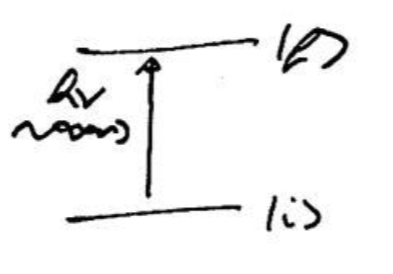
\includegraphics[width=0.7\textwidth]{\currfiledir/tls.png}
\inputtikz{\currfiledir/tls_absorption}

\caption{A light beam induces a transition from $\ket{i}$ to the  $\ket{f}$.}
\end{marginfigure}

Fermi's Golden Rule gives the transition rate from the initial state $\ket{i}$ to the final state $\ket{f}$ caused by the time-dependent perturbation $H'$ to the stationary Hamilton operator $H_0$ as
\begin{equation}
 \Gamma_{i \rightarrow f} = \frac{2 \pi}{\hbar} \, \left| \bra{f} H' \ket{i} \right|^2 \, \rho(E) \quad ,
\end{equation}
where  $\rho(E) = d n / d E = \rho(\omega) / \hbar$ is the density of final states. The idea is that the initial state  $\ket{i}$ is well known, but the outcome of the interaction $\ket{f}$ might have free parameters, for example the direction of the emitted electron or the mode of the absorbed photon. The density of states   $\rho(E)$ thus can describe either electronic or photonic states, or both.




In general, the interaction of a charged particle with an electromagnetic vector potential $\mathbf{A}$ is described by the perturbation
\begin{equation}
 H' = - \frac{i \hbar e}{m} \, \mathbf{A \cdot \nabla}  \quad .
\end{equation}
As the spatial extent of our wavefunctions is small compared to the wavelength of light, we employ the dipole approximation and assume $\exp( i \mathbf{k \cdot r}) \approx 1$ in the plane-wave description of the vector potential. In this way, the  perturbation operator $H'$ simplifies to\sidenote{see \textcite{bransden_joachain} for details}
\begin{equation}
 H' =  e \, \mathbf{E} (t)  \mathbf{\cdot \, r} =  e \,E_0 \,  \mathbf{\hat{x} \cdot \, r} \, \cos(\omega t) \quad ,
\end{equation}
where $\mathbf{\hat{x}} $ is a unit vector defining the polarization direction of the light field. We simplify further by using the rotating-wave approximation and keeping only co-rotating parts\sidenote{More on this in the chapter on Rabi oscillations and the Bloch sphere.} 
\begin{equation}
 \cos(\omega t)
 = \frac{1}{2} \left( e^{i \omega t}+  e^{-i \omega t} \right)
 \approx  \frac{1}{2}  e^{i \omega t} 
\end{equation}
so that 
\begin{equation}
H' =  \frac{ e \,E_0}{2}  \,  \mathbf{\hat{x} \cdot \, r} \,  e^{i \omega t}  \quad .
\end{equation}
%
 We introduce the transition dipole matrix element $\mu_{if}$ as
\begin{equation}
\mathbf{\mu}_{if} = -e \, \bra{f}    \mathbf{r} \ket{i}  \quad .
\end{equation}
It has the units of an electric dipole moment, i.e., charge times distance, and is the central element of an optical transition in quantum mechanics. For practical reasons, one uses the unit of 1 Debye = 1 electron displaced by 0.208 \AA.
With this the matrix element  becomes
\begin{equation}
\left| \bra{f} H' \ket{i} \right|^2 =  \frac{1}{4} E_0^2  \, |\mathbf{\hat{x}} \cdot \mathbf{\mu}_{if} |^2 \quad .
\end{equation}
Plugging everything into Fermi's Golden Rule, we get
\begin{equation}
 \Gamma_{i \rightarrow f} = \frac{\pi}{2 \hbar^2} \,  E_0^2  \, |\mathbf{\hat{x}} \cdot \mathbf{\mu}_{if} |^2 \, \rho(\omega) \quad .
\end{equation}
Now we have to take into account that we use a incoherent multimode light source.\sidenote{The effect of a coherent single mode source will be investigated in the context of Rabi oscillations.} The electric field $E$ is here an incoherent superposition of  modes with the  spectral energy density $u(\omega)$.\sidenote{see \textcite{CT} and \textcite{Fox}   for details}
The total power is thus
\begin{equation}
 \frac{1}{2} \epsilon_0  \, E_0^2  = \int  u(\omega)  \, d\omega \quad .
\end{equation}
The  transition rate is thus 
\begin{equation}
 \Gamma_{i \rightarrow f} =   \frac{\pi  }{\hbar^2 \epsilon_0}  \, |\mathbf{\hat{x}} \cdot \mathbf{\mu}_{if} |^2 \,
\int u(\omega)  
  \rho(\omega)  d \omega \quad .
\end{equation}
As the atomic transition is narrow compared with the light spectrum, the density of states $\rho(\omega)$ selects the transition frequency $\omega_{if}$ 
\begin{equation}
 \Gamma_{i \rightarrow f} =   \frac{\pi  }{\hbar^2 \epsilon_0}  \, |\mathbf{\hat{x}} \cdot \mathbf{\mu}_{if} |^2 \,
 u(\omega_{if})   \quad .
\end{equation}
As each absorption event takes out a photon of energy $\hbar \omega_{if}$, and the energy density moves with the speed of light $c$ we get an integrated absorption cross section $\sigma_{\parallel}$ 
\begin{equation}
 \int \sigma_{\parallel}(\omega) \, d \omega = \frac{ \hbar \omega_{if} \, \bar{\Gamma}_{i \rightarrow f} }{c \, u(\omega_{if})}  = 
  \frac{\pi \omega_{if}}{ \hbar c \, \epsilon_0} \,
 |\mathbf{\mu}_{if} |^2  \quad . \label{eq:abs_sigma_mu}
\end{equation}
The index ${\parallel} $ is necessary, as we dropped the dot product between the direction of the transition dipole moment $\mathbf{\mu}_{if}$ and the polarization direction $\mathbf{\hat{x}}$, assuming optimal parallel orientation. In case of random orientation, i.e., averaging over all possible orientation directions, one finds  a reduction by one third, i.e. $\sigma = 1/3 \sigma_{\parallel} $

We can recover the spectral resolved absorption cross section $\sigma_{\parallel}(\omega)$ by assuming a line-shape function $L(\omega - \omega_0)$ so that 
\begin{equation}
 \sigma_{\parallel}(\omega) =  \frac{\pi \omega_{if}}{ \hbar c \, \epsilon_0} \,
 |\mathbf{\mu}_{if} |^2 \, L(\omega - \omega_{if})
\end{equation}
where the integral over $L$ equals one. Assuming a Lorentzian line shape, the peak value of $L$ equals $1/(\pi \gamma)$ so that
\begin{equation}
 \sigma_{\parallel}(\omega_{if}) =  \frac{\omega_{if}}{ \hbar c \, \epsilon_0 \, \gamma} \,
 |\mathbf{\mu}_{if} |^2  \quad .
\end{equation}
In the chapter on fluorescence we will discuss the relation between the transition dipole moment $|\mathbf{\mu}_{if} |^2 $ and the Einstein $A$ and $B$ coefficients. When spontaneous emission is the only factor to influence the width of the optical transition (as for an atom in vacuum), we find
\begin{equation}
 \gamma = \frac{1}{2} A_{21} = \frac{\omega^3}{6 \pi \hbar c^3 \epsilon_0} |\mathbf{\mu}_{if} |^2  
\end{equation}
so that in this case the absorption cross section reduces to 
\begin{equation}
 \sigma_{\parallel}(\omega_{if}) =  \frac{3}{2 \pi} \, \lambda^2 \quad .
\end{equation}
The absorption cross section of an atom, molecule, nanocrystal is thus limited. However, as only in exceptional cases the line width is Fourier-limited, i.e. limited by the radiative decay, in most cases the absorption cross section is much smaller. The reduction is given by the ratio of the Fourier-limited line width to the observed width of the transition. 


When relating to the  (decadic) molar absorption coefficient $\epsilon(\omega)$ we have to realize that in the more 'atomic' contexts of transition dipole moments and Einstein coefficients, we integrated over the spectral width of the absorption line. We  assumed that the incoming light beam is spectrally much broader than the optical transition. This is not the case for molecular spectra at room temperature. We thus have to integrate also the absorption spectrum over $\omega$ and take into account that $\omega_{if}$ varies, so that
\begin{equation}
 \int_{\text{transition}} \frac{\epsilon(\omega)}{\omega} \, d \omega \, = \, 
  \frac{\pi \, N_A}{ 3 \, \ln(10) \, \hbar c \, \epsilon_0} \,
 |\mathbf{\mu}_{if} |^2
 \, = \, 
  \frac{\hbar\, N_A}{ \ln(10) \, c } \,
B_{12}  \quad .
\end{equation}




\section{Appendix: Thomas-Reiche-Kuhn sum rule}

Taken from Wikipedia. 
%
\begin{align}
& \sum_n (E_n-E_m)\left|\left\langle n | \hat x | m \right\rangle\right|^2 \\
&= \sum_n (E_n-E_m) \left\langle m\right |\hat x\left | n\right\rangle\left\langle n \right| \hat{x}\left | m\right\rangle\\
%
&=\frac{1}{2}\sum_n\left(\left\langle m\right | \hat{x}\hat{H}-\hat{H}\hat{x}\left |n\right\rangle\left\langle n \right | \hat{x}\left | m\right\rangle + \left\langle m \right | \hat{x}\left | n\right\rangle\left\langle n\right | \hat{H}\hat{x}-\hat{x}\hat{H}\left |m\right\rangle \right)\\
%
&=\frac{1}{2}\sum_n \left(\left\langle m\right | \hat{x}\left |n \right\rangle\left\langle n\right | [\hat{H},\hat{x}]\left|m\right\rangle-\left\langle m \right | [\hat{H},\hat{x}]\left | n \right\rangle\left\langle n\right|\hat{x}\left| m \right\rangle \right)\\
%
&=\frac{1}{2}\left( \left\langle m\right | \hat{x}[\hat{H},\hat{x}]\left | m \right\rangle -\left\langle m\right | [\hat{H},\hat{x}]\hat{x}\left |m\right\rangle \right)\\
&=\frac{1}{2} \left( \left\langle m \right | [\hat{x},[\hat{H},\hat{x}]] \left | m \right\rangle \right)\\
%
&= -\frac{i\hbar}{2m_0}\left\langle m\right| [\hat{x},\hat{p}]\left| m \right\rangle\\
%
&= \frac{\hbar^2}{2m_0}
\end{align}
%
using
\begin{equation}
[\hat{H},\hat{x}]=-\frac{i\hbar}{m_0}\hat{p} \quad \text{and} \quad  [\hat{x},\hat{p}]=i\hbar
\end{equation}
The dipole operator $\hat{\mu}$ is proportional to the position operator $\hat{x}$. The sum over all $|\mathbf{\mu}_{if}|^2$ starting from the same state $i$ is thus constant.

\section{Appendix: Units }

mass $M$, time $T$, length $L$, current $i$, particle number $mol$

\begin{tabular}{rl}
   $\epsilon_0$  & $i^2 T^4 / M L^3$ \\
    field $E_0$ & $M L / i T^3$ \\
    energy & $M L^2 / T^2$ \\
    $\mu_{if}$ & $ L i T$ \\
    $\omega$ & $1/T$ \\
    $u(\omega)$ & $M / T L$ \\
    $\hbar$ & $ M L^2 / T$ \\
    $\rho(\omega) $ & $T$ \\
    $\Gamma_{if}$ & $ 1/T$ \\
    $B_{12}$ & $ L / M$ \\
  $\epsilon(\omega)$ & $L^2 / mol$
\end{tabular}

\printbibliography[segment=\therefsegment,heading=subbibliography]
